\chapter{Background}
\label{ch:background}

This chapter provides the background knowledge relevant for the thesis work. It
will initially discuss graph and related problems (\autoref{sec:signed_graphs_and_density}) which are significant in the
following used methodologies, as well as concepts of computational complexity
(\autoref{sec:computational_complexity_and_approximability}) and Linear
Programming (\autoref{sec:linear_and_mixed_integer_programming}).

\section{Signed graphs and density}%
\label{sec:signed_graphs_and_density}

\section{Computational complexity and \\approximability}%
\label{sec:computational_complexity_and_approximability}

Complexity Theory deals with the study of the intrinsic complexity of
computational tasks; more specifically it mainly aims at determining the
complexity of any given task. It also elaborates on the relationships between
the complexity of different problems, for example proving that 2 problems are
computationally equivalent\cite{9780521884730}, through a notion called
\emph{reduction}.

\subsection{Complexity classes}%
\label{par:complexity_classes}

According to their complexity, problems can be divided in different groups
\cite{DemaineFall2014}.

\paragraph{$\mathcal{P} $}%
\label{par:p}
is the set of problems which can be solved in polynomial time in the size $n$ of
the problem, i.e. $n^{O(1)} $. In this set there are problems such as Linear
Programming Models \cite{KHACHIYAN198053}\cite{Karmarkar1984}, finding whether
or not a graph is connected \cite{9780521884730}.

\paragraph{$\mathcal{NP} $}%
\label{par:np} is the set of problems whose solution can be verified in
polynomial time in the size $n$ of the problem, i.e. $n^{O(1)} $.

According to these definition it is easy to see that $\mathcal{P} \subseteq
	\mathcal{NP} $. A common $\mathcal{NP} $ problem is factoring, i.e. finding a
prime factor $p$ of a number $N$ in a given interval \cite{SanjeevArora2017}.

\paragraph{$\mathcal{NP} $-Hard}%
\label{par:_np_hard} is the set of problems that are \emph{at least as hard} as
any other problem in $\mathcal{NP} $. Some well-known $\mathcal{NP} $-Hard
problems are the $\textsc{Sat}$ (deciding whether a boolean formula can be
satisfied or not) and the $\textsc{MaxClique}$ (finding the biggest complete
subgraph), as shown is a famous paper by Karp \cite{Miller1972} (see
\autoref{fig:tex/img/post_vaccine_social_scheduling} ).

\begin{figure}[]
	\centering
	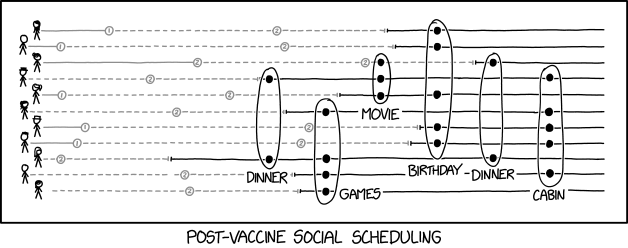
\includegraphics[width=0.8\linewidth]{tex/img/post_vaccine_social_scheduling.png}
	\caption{\emph{As if this problems weren't $\mathcal{NP} $-Hard enough}.
		Post-vaccine social scheduling may be $\mathcal{NP} $-Hard \cite{Munroe}}%
	\label{fig:tex/img/post_vaccine_social_scheduling}
\end{figure}

\paragraph{$\mathcal{NP} $-Complete}%
\label{par:_np_hard} is the set of problems in $\mathcal{NP} $-Hard that are
also in $\mathcal{NP} $. Intuitively these correspond the most difficult
problems to solve in $\mathcal{NP} $. The number of problems which are known to
be in this set is in the order of a thousand \cite{SanjeevArora2017}.

\subsection{$\mathcal{P} $ vs $\mathcal{NP}$}%
\label{sub:_p_vs_np_}

A fundamental question in Computational Complexity is wheter $\mathcal{P} =
	\mathcal{NP} $: this corresponds to asking if there exist some problems for
which the solution can be checked efficiently (i.e. in polynomial time) but
for which it is not easy to find the solution, given the problem
instance \cite{9780521884730}.

If this is the case, as it is mostly accepted among the algorithm designers
\cite{Erickson2019} (on this assumption also Modern Criptography heavily relies
\cite{9780521884730}), then
$\mathcal{P} \neq \mathcal{NP} $, which will then
bring to a representation of the compexity classes as depicted in
\autoref{fig:tex/img/complexity-diagram}. But, in fact, in the last decades
there has been little or no progress towards this proof \cite{Erickson2019}.

\begin{figure}[]
	\centering
	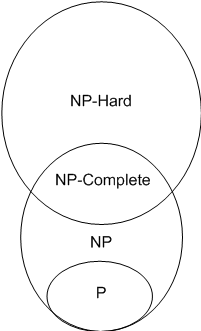
\includegraphics[width=0.3\linewidth]{tex/img/complexity-diagram.png}
	\caption{Venn diagram for the complexity classes if $\mathcal{P} \neq
			\mathcal{NP} $ \cite{article}}%
	\label{fig:tex/img/complexity-diagram}
\end{figure}

\subsection{Optimization Problems}%
\label{sub:optimization_problems}



\section{Linear and Mixed Integer Programming}%
\label{sec:linear_and_mixed_integer_programming}
